\section{Causal Bayesian Networks}

In all following discussion, we assume the observed data represented by $\RV{X}$ is a sequence of independent and identically distributed random variables $\RV{X}=(\RV{X}_t)_{t\in T}$. We identify distributions over the sequence $\RV{X}$ with distributions over the initial observation $\RV{X}_0$ and subsequently drop the subscript.

There is a natural identification of a causal Bayesian network (CBN) associated with a graph $\mathcal{G}$ and a causal theory $\mathscr{T}_{\mathcal{G}}$ where we consider \emph{do}-interventions defined with respect to the CBN to correspond to decisions in the causal theory. The CBN convention is to denote an interventional distribution with $P(\cdot|do(\RV{X}^i=a))$ notation. Here we associate every allowable intervention with the decision space $(D,\mathcal{D})$ equipped with random variables $\{\RV{D}^i\}_{i\in[N]}$ such that for $y\in D$, $P^y(\cdot) := P(\cdot|[do(\RV{X}^j=\RV{D}^i(y))]_{i\in N})$. The special element $*$ corresponds to a passive intervention which is denoted by the absence of a $do()$ statement in regular CBN notation.

\begin{definition}[Causal Bayesian Network]\label{def:CBN}
Consider a directed acyclic graph $\mathcal{G}$ with nodes $\mathbf{X}=\{\RV{X}^i|i\in [N]\}$, a measurable space $(E,\mathcal{E})$ and a set of random variables $\RV{X}^i:E\to X^i$ and $X=\times_{i\in[N]} X^i$ along with decision space $(D,\mathcal{D})$ and random variables $\{\RV{D}^i\}_{i\in [N]}$ where $\RV{D}^i:D\to X^i\cup\{*\}$.

Given any $y\in D$ let $S(y)\subset[N]$ be the set of all indices $i$ such that $\RV{D}^i(y)\neq *$. Let $\mathscr{H}_\mathcal{G}\subset\Delta(\mathcal{X})$ be the set of distributions compatible with $\mathcal{G}$. Given arbitrary $\mu\in \mathscr{H}_\mathcal{G}$ and $y\in D$ the $\mathcal{G},\mu,y$-interventional distribution denoted $\mu^{\mathcal{G},y}$ is given by the following three conditions:
\begin{enumerate}
    \item $\mu^{\mathcal{G},y}$ is compatible with $\mathcal{G}$
    \item For all $i\in S(y)$, $\mu^{\mathcal{G},y}F_{\RV{X}^i}=\delta_{\RV{D}^i(y)} F_{\RV{X}^i}$
    \item For all $i\not \in S(y)$, $\mu^{\mathcal{G},y}_{\PA{\mathcal{G}}{\RV{X}^i}} F_{\RV{X}^i}=\mu_{\PA{\mathcal{G}}{\RV{X}^i}}F_{\RV{X}^i} $, $\mu^{\mathcal{G},y}$-almost surely
\end{enumerate}
\end{definition}

$\PA{\mathcal{G}}{\RV{X}^i}$ are the parents of $\RV{X}^i$ with respect to the graph $\mathcal{G}$ and $\mu_{\PA{\mathcal{G}}{\RV{X}^i}}$ is the conditional probability with respect to $\mu$ and the $\sigma$-algebra generated by the set $\PA{\mathcal{G}}{\RV{X}^i}$. Recall that $\mu \splitter{0.15}(\otimes_{i\not\in S(y)} F_{\RV{X}^i})$ is the joint distribution of $\{\RV{X}^i|i\in S(y)\}$.

To establish that the map $\kappa^{\mathcal{G},\mu}:D\to \Delta(\mathcal{X})$ given by $y\mapsto \mu^{\mathcal{G},y}$ is a consequence map, we must shown that it is measurable with respect to the $\sigma$-algebra generated by the set of variables $\RV{D}^i$; this is shown by Theorem \ref{th:cbn_MK} provided in Appendix \ref{app:cbn_ct}. Defining $\mathscr{H}_{\mathcal{G}}\subset\Delta(\mathcal{X})$ to be the set of distributions compatible with $\mathcal{G}$, the set of pairs $\{(\mu, \kappa^\mu)|\mu\in \mathscr{H}_{\mathcal{G}}\}$ is the causal theory $\mathscr{T}_\mathcal{G}$.

\subsection{Extending the theory induced by a CBN}

The causal theory $T_{\mathcal{G}}$ defined above associates a consequence with every probability distribution compatible with $\mathcal{G}$ but not every probability distribution in $\Delta(\mathcal{X})$ (this follows from condition 1 of Definition \ref{def:CBN}). It is arguably not reasonable to assume \emph{a priori} that the conditional independences implied by $\mathcal{G}$ hold in the observed data. We therefore need to extend the theory $\mathscr{T}_{\mathcal{G}}$ to account for the possibility of incompatible distributions. There are many meaningfully different choices for how this may be done as shown by Example \ref{ex:extn_cbn}.

\begin{example}[Extension of a CBN]\label{ex:extn_cbn}

Consider the graph $\mathcal{G}=$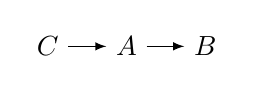
\begin{tikzpicture}[baseline=-1.5mm,-latex]
\node (C) {$C$};
\node [right of = C] (A) {$A$};
\node [right of = A] (B) {$B$};
\draw (C) -- (A);
\draw (A) -- (B);
\end{tikzpicture}, which implies a single conditional independence: $\RV{C}\CI \RV{B}|\RV{A}$.

Suppose the three associated random variables $\RV{A}$, $\RV{B}$ and $\RV{C}$ each take values in $\{0,1\}$ and suppose (unrealistically) we know all $\mu$ in the set of possible joint distributions $\mathscr{H}$ share the marginal distribution $\mu F_{\RV{B}} := \zeta$ and the conditional distribution $\mu_{\{\RV{A}\}} F_{\RV{B}} = \iota$ and $\RV{C}$ is ``almost'' independent of $\RV{B}$ given $\RV{A}$:
\begin{align}
    \max_{x\in\{0,1\}^3,y\in\{0,1\}}\left|\mu_{\{\RV{A},\RV{C}\}} F_{\RV{B}}(x;\{y\}) - \iota(x;\{y\}) \right| &< \epsilon \label{eq:app_ci}
\end{align}

Suppose that only interventions on $\RV{A}$ are possible and the problem supplies a utility such that, overloading $\RV{B}$, $U(\xi)=\mathbb{E}_[\xi][\RV{B}]$. For convenience, we restrict our attention to the subset of decisions $D'=\{y|\RV{D}_\RV{B}(y)=\RV{D}_\RV{C}(y)=*\}$ and consequence maps marginalised over $\RV{A}$ and $\RV{C}$. Define $\kappa^{\mathcal{G}}$ by
\begin{align}
    \kappa^{\mathcal{G}}(y;Z) := \begin{cases} \iota(\RV{D}_A(y);Z) & \RV{D}_\RV{A}(y) \neq *\\
                                              \zeta(Z) & \RV{D}_\RV{A}(y) = *\end{cases}
\end{align}

It can be verified that the causal theory $\mathscr{T}_{\mathcal{G}}$ induced by $\mathcal{G}$ and the set of compatible distributions $\mathscr{H}_\mathcal{G}\subset\mathscr{H}$ is the set of pairs $\{(\nu,\kappa^{\mathcal{G}} )|\nu\in \mathscr{H}_{\mathcal{G}}\}$.

Consider two options for extending this to distributions $\nu\in \mathscr{H}$ but not in $\mathscr{H}_{\mathcal{G}}$, noting that one could imagine many possibilities: $\mathscr{T}_{\mathcal{G}}^\subset$ is the union of causal theories given by all graphs $\mathcal{G}'$ on $\{A, B, C\}$ such that $\mathcal{G}\subset \mathcal{G}'$ (in this case, just $\mathcal{G}$ and 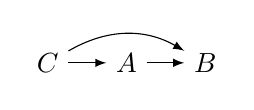
\begin{tikzpicture}[baseline=-1.5mm,-latex]
\node (C) {$C$};
\node [right of = C] (A) {$A$};
\node [right of = A] (B) {$B$};
\draw (C) -- (A);
\draw (A) -- (B);
\draw (C) to [bend left] (B);
\end{tikzpicture}), and  $\mathscr{T}_{\mathcal{G}}^\circ$ is the union of causal theories given by the all DAGs on the set of nodes $\{\RV{A}, \RV{B}, \RV{C}\}$.

The theory $\mathscr{T}_{\mathcal{G}}^\subset$ is given by $\mathscr{T}_{\mathcal{G}}\cup\{(\nu,\eta^\nu )|\nu \in \mathscr{H}\setminus\mathscr{H}_\mathcal{G}\}$ where 
\begin{align}
    \eta^\nu:=\begin{cases}(y;Z)\mapsto \sum_{c\in\{0,1\}} \nu F_{\RV{C}}(\{c\}) \nu_{\{\RV{A},\RV{C}\}} F_{\RV{B}}(\RV{D}_A(y),c;Z) &\RV{D}_A(y)\neq *\\
    \zeta(Z) &\RV{D}_A(y)=*\end{cases}
\end{align}

$\mathscr{T}_{\mathcal{G}}^\circ$ is the set of states associated with three types of graph: those featuring no arrow \begin{tikzpicture}[baseline=-1.5mm,-latex]
\node (A) {$A$};
\node [right of = A] (B) {$B$};
\draw (A) -- node[strike out,draw,-]{} (B);
\end{tikzpicture}, those featuring 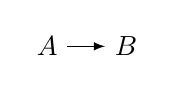
\begin{tikzpicture}[baseline=-1.5mm,-latex]
\node  (A) {$A$};
\node [right of = A] (B) {$B$};
\draw (A) -- (B);
\end{tikzpicture} but not 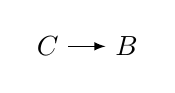
\begin{tikzpicture}[baseline=-1.5mm,-latex]
\node  (C) {$C$};
\node [right of = C] (B) {$B$};
\draw (C) -- (B);
\end{tikzpicture} and 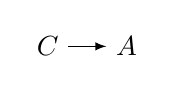
\begin{tikzpicture}[baseline=-1.5mm,-latex]
\node  (C) {$C$};
\node [right of = C] (A) {$A$};
\draw (C) -- (A);
\end{tikzpicture} and the graph 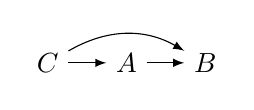
\begin{tikzpicture}[baseline=-1.5mm,-latex]
\node (C) {$C$};
\node [right of = C] (A) {$A$};
\node [right of = A] (B) {$B$};
\draw (C) -- (A);
\draw (A) -- (B);
\draw (C) to [bend left] (B);
\end{tikzpicture}. These possibilities yield $\mathscr{T}_{\mathcal{G}}^\circ=\mathscr{T}_{\mathcal{G}}^\subset\cup\{(\nu,y\mapsto \zeta)|\nu \in \mathscr{H}\setminus\mathscr{H}_\mathcal{G}\}$.

By \ref{eq:app_ci}, $|\eta(x;\{y\})-\iota(x;\{y\})|<\epsilon$ for all $x\in A\cup\{*\}$ and $y\in B$ and therefore for $J\in \mathscr{J}$, $|U(\mu J\splitter{0.1} (I_D\otimes \eta)) - U(\mu J\splitter{0.1} (I_D\otimes \iota))|<\epsilon$. Therefore a small $\epsilon$ ensures $\mathscr{T}^\subset_{\mathcal{G}}$ yields a risk set ``close'' to $\mathscr{T}_{\mathcal{G}}$. On the other hand, $|\iota(x;\{y\})-\zeta(\{y\})|$ is independent of $\epsilon$, so $\mathscr{T}^\circ_{\mathcal{G}}$ yields a larger risk set independent of $\epsilon$.

\end{example}

It is possible to extend the theory $\mathscr{T}_{\mathcal{G}}$ to theories with very different properties even where the extension is very slight. There is no apparent consensus on how ``near-misses'' should be treated in the context of graph learning. Theoretical justifications of the faithfulness assumption may work with exact conditional independences \citep{meek_strong_1995}, while in at least one practical application it was found desirable to accept conditional independences unless the observed dependence exceeded a significance level $\alpha=0.01$ [\cite{maathuis_predicting_2010}, supplementary material], a setting that would under a wide variety of assumptions lead to many false positives. More broadly, many statisticians are of the opinion that it is very unusual for exact conditional independence to ever hold \citep{gelman_bayesian_2010,meehl_theory-testing_1967,berkson_difficulties_1938}